\section{Learning Vector Quantization}
\label{sect:learning-vector-quantization}
Der initiale Ansatz ist \textit{vector quantization}, welcher als erstes besprochen wird. Die Weiterentwicklung des vector quantization ist \textit{learning vector quantization}, welche danach behandelt wird.

\subsection{Vector Quantization}
\label{ssect:vector-quantization}
Die Idee hinter vector quantization ist, dass der \textit{data space} mit einer kleinen Anzahl an \textit{prototype vectors} $U = u_1, u_2, ..., u_k$ beschrieben wird. Jeder prototype vector repräsentiert eine Klasse ($k$ Klassen). Dazu muss jeder Input Vektor $X = x_1, x_2, ..., x_m$ einem der Vektoren in $U$ zugewiesen werden. Die prototype vectors $U$ sind in einem \textit{codebook} zusammengefasst. Vector Quantization ist unsupervised.

\subsubsection{Applications}
\label{sssect:vq-application}
\begin{itemize}
	\item multimedia compression (storage and transmission)
	\item dimensionality reduction
	\item classification
\end{itemize}

\subsubsection{Training}
\label{ssect:vq-training}
Beim Trainieren werden die Input Vektoren mittels einem geeignetem Distanzmaß $d$ und einem Clustering Algorithmus unterteilt. Daraus ergeben sich die Anzahl an Klassen und somit auch direkt die Anzahl an Codebuch Einträgen. Die Vektoren im Codebuch sind die \textit{centroids} der einzelnen Regionen.
Bei der eigentlichen Klassifikation (Encoding) wird für einen Input Vektor die Distanz zu den Codebuch Einträgen berechnet und bei der minimalen Entfernung der Index des prototype vectors gemerkt (bzw. übermittelt).
Beim Decoding wird anhand des Index der jeweilige prototype vector ausgewählt und repräsentiert somit den Input Vektor. Der Fehler hierbei ist das Distanzmaß des Input Vektors und des prototype vectors.
\begin{figure}[h]
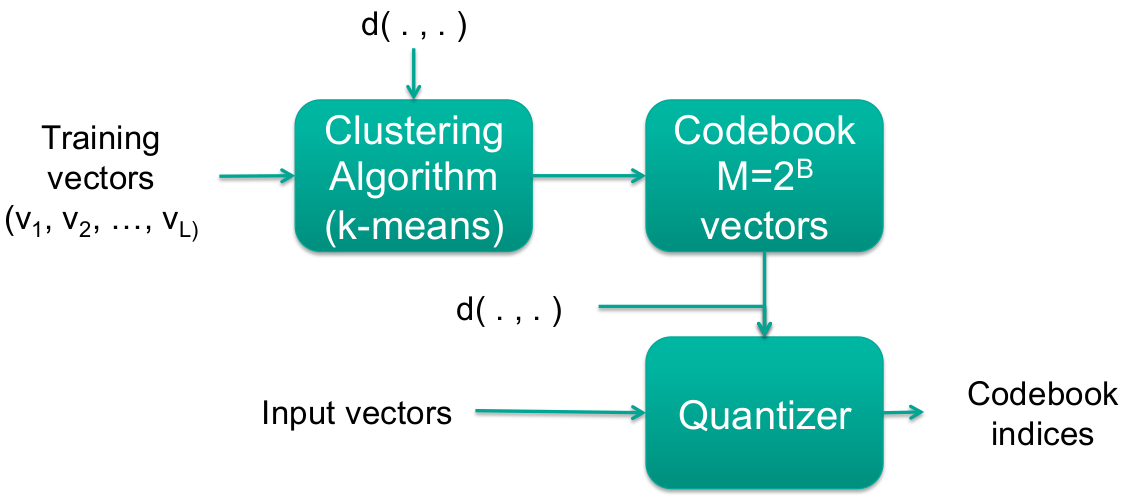
\includegraphics[scale=0.3]{vector-quantization-training}
\end{figure}

\subsection{Learning Vector Quantization}
\label{ssect:learning-vector-quantization}
Da wir nun über Labels verfügen (also wissen in welche Klasse der Input Vektor gehört), lassen sich nun Wahtscheinlichkeitsverteilungen nutzen:
\begin{itemize}
	\item $P(S_k)$: a prior Wahrscheinlichkeit der Klasse $S_k$
	\item $p(x|x \in S_k) $: bedingte Wahrscheinlichkeitsdichte 
	\item discriminant functions: $\delta_k(x) = p(x|x \in S_k) P(S_k)$
	\item rate of misclassification minimized if: $\delta_c(x) = max_k\{\delta_k(x)\}$
\end{itemize}
Prinzipiell weisen wir mehrere prototype vectors den einzelnen Klasse zu. Ein Input Vector erhält die selbe Klasse wie der prototype vector, an dem der Input Vektor am nähsten ist. Da wir nun aber mehrere prototype vectors je Klasse haben, müssen wir entscheiden, welcher der \textit{winning codebook entry} ($c$ ist der Index) ist. Die einzelnen Algorithmen unterscheiden sich in dieser Wahl:
\subsubsection{LVQ1}
\label{sssect:vq-lvq1}
$c = argmin_i\{||x - m_i||\}$: Index des prototype vectors\\
Learning rules:
\begin{itemize}
	\item $m_c(t + 1) = m_c(t) + \alpha(t)[x(t) - m_c(t)]$: $x$ und $m_c$ selbe Klasse
	\item $m_c(t + 1) = m_c(t) - \alpha(t)[x(t) - m_c(t)]$: $x$ und $m_c$ unterschiedliche Klasse
	\item $m_c(t + 1) = m_i(t)$: für $i \neq c$
\end{itemize}

\subsubsection{LVQ2}
\label{sssect:vq-lvq2}
Die Klassifizierung ist die selbe wie bei LVQ1. Das updaten ist anders:
\begin{itemize}
	\item $m_i$ und $m_j$ sind die nähsten Nachbarn von $x$ und werden simulaten geupdated.
	\item $x$ muss in ein ''window'' um $m_i$ und $m_j$ fallen.
	\item $d_i$ und $d_j$ sind die Distanzen (z.B. euklidien) zwischen $x$ und $m_i$ und $m_j$
	\item $min \left(\frac{d_i}{d_j}, \frac{d_j}{d_i}\right) > s$ where $s = \frac{1 - w}{1 + w}$ (recommended window: 0.2 to 0.3)
\end{itemize}


Ergänzungen:
$m_i$ ist der Gewinner (falsche klasse)
$m_j$ zweiter gewinner, richtige klasse -> dann updaten
$\alpha$ die Lernrate wird kleiner und kleiner

\subsubsection{LVQ2.1}
\label{sssect:vq-lvq2.1}


\subsubsection{LVQ3}
\label{sssect:vq-lvq3}



Ergänzen:
- die Frage ist welches k das korrekte ist. Zur Not kann man die Distortion betrachten und ein anderen k wählen +-
- $delta_k$ = wkeit das x zu $s_k$ gehört
- stopping rule -> fehler kleine genug oder anzahl iteration erreicht
\subsubsection{OLVQ}
\label{sssect:vq-olvq}

\newpage